\exo{Raisonner}{VolumeComplexe1}

Tous les angles sont droits. Calculer le volume du solide ci-dessous.

\begin{figure}[H]
    \centering
    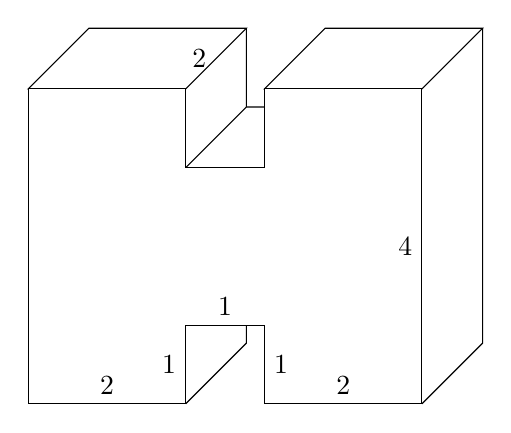
\begin{tikzpicture}
        \draw (0,4,0) --(2,4,0) -- node [midway,left] {2}  (2,4,-2) -- (0,4,-2)--cycle; %Face haute gauche
        \draw (3,4,0) --(5,4,0) -- (5,4,-2) -- (3,4,-2)--cycle; %Face haute droite
        \draw (5,0,0) -- (5,0,-2) -- (5,4,-2); %Cote droit
        \draw (2,0,0) -- (2,0,-2) -- (2,4,-2); %A faire en cavaliere
        \draw [fill=white] (2,3,0) --(2,3,-2) -- (3,3,-2)--(3,3,0); %Millieu haut
        \draw [fill=white] (0,0,0) --node [midway,above] {2} (2,0,0)-- node [midway,left] {1}(2,1,0)--node [midway,above] {1} (3,1,0)--node [midway,right] {1} (3,0,0)--node [midway,above] {2} (5,0,0)--node [midway,left] {4}(5,4,0)--(3,4,0)--(3,3,0)--(2,3,0)--(2,4,0)--(0,4,0)--cycle; %Face avant
    \end{tikzpicture}
\end{figure}